% !TeX spellcheck = de_DE
% !TeX program = make
% Dieses Dokument muss mit PDFLatex gesetzt werden
% Vorteil: Grafiken koennen als jpg, png, ... verwendet werden
%          und die Links im Dokument sind auch gleich richtig
%
%Ermöglicht \\ bei der Titelseite (z.B. bei supervisor)
%Siehe https://github.com/latextemplates/uni-stuttgart-cs-cover/issues/4
\RequirePackage{kvoptions-patch}

%English:
\let\ifdeutsch\iffalse
\let\ifenglisch\iftrue

%German:
%\let\ifdeutsch\iftrue
%\let\ifenglisch\iffalse

%
\ifenglisch
	\PassOptionsToClass{numbers=noenddot}{scrbook}
\else
	%()Aus scrguide.pdf - der Dokumentation von KOMA-Script)
	%Nach DUDEN steht in Gliederungen, in denen ausschließlich arabische Ziffern für die Nummerierung
	%verwendet werden, am Ende der Gliederungsnummern kein abschließender Punkt
	%(siehe [DUD96, R3]). Wird hingegen innerhalb der Gliederung auch mit römischen Zahlen
	%oder Groß- oder Kleinbuchstaben gearbeitet, so steht am Ende aller Gliederungsnummern ein
	%abschließender Punkt (siehe [DUD96, R4])
	\PassOptionsToClass{numbers=autoendperiod}{scrbook}
\fi

%Warns about outdated packages and missing caption delcarations
%See https://www.ctan.org/pkg/nag
\RequirePackage[l2tabu, orthodox]{nag}

%Neue deutsche Trennmuster
%Siehe http://www.ctan.org/pkg/dehyph-exptl und http://projekte.dante.de/Trennmuster/WebHome
%Nur für pdflatex, nicht für lualatex
\RequirePackage{ifluatex}
\ifluatex
%do not load anything
\else
	\ifdeutsch
		\RequirePackage[ngerman=ngerman-x-latest]{hyphsubst}
	\fi
\fi

\documentclass[
               fontsize=12pt, %Default: 11pt, bei Linux Libertine zu klein zum Lesen
% BEGINN: Optionen für typearea
               paper=a4,
               twoside,  % fuer die Betrachtung am Schirm ungeschickt
               BCOR=3mm, % Bindekorrektur
               DIV=13,   % je höher der DIV-Wert, desto mehr geht auf eine Seite. Gute werde sind zwischen DIV=12 und DIV=15
               headinclude=true,
               footinclude=false,
% ENDE: Optionen für typearea
%               titlepage,
               bibliography=totoc,
%               idxtotoc,   %Index ins Inhaltsverzeichnis
%                liststotoc, %List of X ins Inhaltsverzeichnis, mit liststotocnumbered werden die Abbildungsverzeichnisse nummeriert
               headsepline,
               cleardoublepage=empty,
               parskip=half,
%               draft    % um zu sehen, wo noch nachgebessert werden muss - wichtig, da Bindungskorrektur mit drin
               final   % ACHTUNG! - in pagestyle.tex noch Seitenstil anpassen
               ]{scrbook}


%%%
% Beschreibung:
% In dieser Datei werden zuerst die benoetigten Pakete eingebunden und
% danach diverse Optionen gesetzt. Achtung Reihenfolge ist entscheidend!
%
%%%


%%%
% Styleguide:
%
% Ein sehr kleiner Styleguide. Packages werden in Blöcken organisiert.
% Ein Block beginnt mit drei % in einer Zeile, dann % <Blocküberschrift>, dann
% eine Liste der möglichen Optionen und deren Einstellungen, Gründe und Kommentare
% eine % Zeile in der sonst nichts steht und dann wieder %%% in einer Zeile.
%
% Zwischen zwei Blöcken sind 2 Leerzeilen!
% Zu jedem Paket werden soviele Optionen wie möglich/nötig angegeben
%
%%%

%%%
% Required for recent version of komascript, as this template does not use the most recent commands of KOMAScript
\usepackage{scrhack}
%%%

%%%
% Codierung
% Wir sind im 21 Jahrhundert, utf-8 löst so viele Probleme.
%
% Mit UTF-8 funktionieren folgende Pakete nicht mehr. Bitte beachten!
%   * fancyvrb mit §
%   * easylist -> http://www.ctan.org/tex-archive/macros/latex/contrib/easylist/
\ifluatex
%no package loading required
\else
\usepackage[utf8]{inputenc}
\fi
%
%%%

%%%
%Parallelbetrieb tex4ht und pdflatex
\makeatletter
\@ifpackageloaded{tex4ht}{\def\iftex4ht{\iftrue}}
                         {\def\iftex4ht{\iffalse}}
\makeatother
%%%


%%%
%Farbdefinitionen
\usepackage[hyperref,dvipsnames]{xcolor}
%

%%%
% Required for custom acronyms/glossaries style
% Left aligned Columns in tables with fixed width
% see http://tex.stackexchange.com/questions/91566/syntax-similar-to-centering-for-right-and-left
\usepackage{ragged2e}
%%%

%%%
% Abkürzungsverzeichnis
\usepackage{scrwfile} % Wichtig, ansonsten erscheint "No room for a new \write"
% siehe http://www.dickimaw-books.com/cgi-bin/faq.cgi?action=view&categorylabel=glossaries#glsnewwriteexceeded
\usepackage[acronym,indexonlyfirst,nomain]{glossaries}
\ifdeutsch
\renewcommand*{\acronymname}{Abkürzungsverzeichnis}
\else
\renewcommand*{\acronymname}{List of Abbreviations}
\fi
\renewcommand*{\glsgroupskip}{}
%
% Removed Glossarie as a table as a quick fix to get the template working again
% see http://tex.stackexchange.com/questions/145579/how-to-print-acronyms-of-glossaries-into-a-table
%
\makenoidxglossaries
%%%


%%%
% Neue deutsche Rechtschreibung und Literatur statt "Literature", Nachfolger von ngerman.sty
\ifdeutsch
% letzte Sprache ist default, Einbindung von "american" ermöglicht \begin{otherlanguage}{amercian}...\end{otherlanguage} oder \foreignlanguage{american}{Text in American}
% see also http://tex.stackexchange.com/a/50638/9075
\usepackage[american,ngerman]{babel}
% Ein "abstract" ist eine "Kurzfassung", keine "Zusammenfassung"
\addto\captionsngerman{%
	\renewcommand\abstractname{Kurzfassung}%
}
\else
%
%
% if you are writing in english
% last language is the default language
\usepackage[ngerman,american]{babel}
\fi
%
%%%

%%%
% Anführungszeichen
% Zitate in \enquote{...} setzen, dann werden automatisch die richtigen Anführungszeichen verwendet.
\usepackage{csquotes}
%%%


%%%
% erweitertes Enumerate
\usepackage{paralist}
%
%%%


%%%
% fancyheadings (nicht nur) fuer koma
\usepackage[automark]{scrlayer-scrpage}
%
%%%


%%%
%Mathematik
%
\usepackage[]{amsmath} % Viele Mathematik-Sachen: Doku: /usr/share/doc/texmf/latex/amsmath/amsldoc.dvi.gz
\PassOptionsToPackage{fleqn,leqno}{amsmath} % options must be passed this way, otherwise it does not work with glossaries
%fleqn (=Gleichungen linksbündig platzieren) funktioniert nicht direkt. Es muss noch ein Patch gemacht werden:
%\addtolength\mathindent{1em}%work-around ams-math problem with align and 9 -> 10. Does not work with glossaries, No visual changes.
\usepackage{mathtools} %fixes bugs in AMS math
%
%for theorems, replacement for amsthm
\usepackage[amsmath,hyperref]{ntheorem}
\theorempreskipamount 2ex plus1ex minus0.5ex
\theorempostskipamount 2ex plus1ex minus0.5ex
\theoremstyle{break}
\newtheorem{definition}{Definition}[section]
%
%%%


%%%
% Intelligentes Leerzeichen um hinter Abkürzungen die richtigen Abstände zu erhalten, auch leere.
% siehe commands.tex \gq{}
\usepackage{xspace}
%Macht \xspace und \enquote kompatibel
\makeatletter
\xspaceaddexceptions{\grqq \grq \csq@qclose@i \} }
\makeatother
%
%%%


%%%
% Anhang
\usepackage{appendix}
%[toc,page,title,header]
%
%%%


%%%
% Grafikeinbindungen
\usepackage{graphicx}%Parameter "pdftex" unnoetig
\graphicspath{{\getgraphicspath}}
\newcommand{\getgraphicspath}{graphics/}
%
%%%


%%%
% Enables inclusion of SVG graphics - 1:1 approach
% This is NOT the approach of http://www.ctan.org/tex-archive/info/svg-inkscape,
% which allows text in SVG to be typeset using LaTeX
% We just include the SVG as is
\usepackage{epstopdf}
\epstopdfDeclareGraphicsRule{.svg}{pdf}{.pdf}{%
  inkscape -z -D --file=#1 --export-pdf=\OutputFile
}
%
%%%


%%%
% Enables inclusion of SVG graphics - text-rendered-with-LaTeX-approach
% This is the approach of http://www.ctan.org/tex-archive/info/svg-inkscape,
\newcommand{\executeiffilenewer}[3]{%
\IfFileExists{#2}
{
%\message{file #2 exists}
\ifnum\pdfstrcmp{\pdffilemoddate{#1}}%
{\pdffilemoddate{#2}}>0%
{\immediate\write18{#3}}
\else
{%\message{file up to date #2}
}
\fi%
}{
%\message{file #2 doesn't exist}
%\message{argument: #3}
%\immediate\write18{echo "test" > xoutput.txt}
\immediate\write18{#3}
}
}
\newcommand{\includesvg}[1]{%
\executeiffilenewer{#1.svg}{#1.pdf}%
{
inkscape -z -D --file=\getgraphicspath#1.svg %
--export-pdf=\getgraphicspath#1.pdf --export-latex}%
\input{\getgraphicspath#1.pdf_tex}%
}


%%%
\usepackage{siunitx}
%%%

%%%
% Tabellenerweiterungen
\usepackage{array} %increases tex's buffer size and enables ``>'' in tablespecs
\usepackage{longtable}
\usepackage{dcolumn} %Aligning numbers by decimal points in table columns
\ifdeutsch
	\newcolumntype{d}[1]{D{.}{,}{#1}}
\else
	\newcolumntype{d}[1]{D{.}{.}{#1}}
\fi

%
%%%

%%%
% Eine Zelle, die sich über mehrere Zeilen erstreckt.
% Siehe Beispieltabelle in Kapitel 2
\usepackage{multirow}
%
%%%

%%%
%Fuer Tabellen mit Variablen Spaltenbreiten
%\usepackage{tabularx}
%\usepackage{tabulary}
%
%%%


%%%
% Links verhalten sich so, wie sie sollen
\usepackage{url}
%
%Use text font as url font, not the monospaced one
%see comments at http://tex.stackexchange.com/q/98463/9075
\urlstyle{same}
%
%Hint by http://tex.stackexchange.com/a/10419/9075
\makeatletter
\g@addto@macro{\UrlBreaks}{\UrlOrds}
\makeatother
%
%%%


%%%
% Index über Begriffe, Abkürzungen
%\usepackage{makeidx} makeidx ist out -> http://xindy.sf.net verwenden
%
%%%

%%%
%lustiger Hack fuer das Abkuerzungsverzeichnis
%nach latex durchlauf folgendes ausfuehren
%makeindex ausarbeitung.nlo -s nomencl.ist -o ausarbeitung.nls
%danach nochmal latex
%\usepackage{nomencl}
%    \let\abk\nomenclature %Deutsche Ueberschrift setzen
%          \renewcommand{\nomname}{List of Abbreviations}
%        %Punkte zw. Abkuerzung und Erklaerung
%          \setlength{\nomlabelwidth}{.2\hsize}
%          \renewcommand{\nomlabel}[1]{#1 \dotfill}
%        %Zeilenabstaende verkleinern
%          \setlength{\nomitemsep}{-\parsep}
%    \makenomenclature
%
%%%

%%%
% Logik für Tex
\usepackage{ifthen} %fuer if-then-else @ commands.tex
%
%%%


%%%
%
\usepackage{listings}
%
%%%

%%%
% To add package to enable restructuring of tables
\usepackage[export]{adjustbox}
\usepackage{lipsum}
% To add package to enable subfigures
%\usepackage{subfigure}
%
%%%

%%%
%Alternative zu Listings ist fancyvrb. Kann auch beides gleichzeitig benutzt werden.
\usepackage{fancyvrb}
%\fvset{fontsize=\small} %Groesse fuer den Fliesstext. Falls deaktiviert: \normalsize
%Funktioniert mit UTF-8 nicht mehr
%\DefineShortVerb{\§} %Somit kann im Text ganz einfach |verbatim| text gesetzt werden.
\RecustomVerbatimEnvironment{Verbatim}{Verbatim}{fontsize=\footnotesize}
\RecustomVerbatimCommand{\VerbatimInput}{VerbatimInput}{fontsize=\footnotesize}
%
%%%


%%%
% Bildunterschriften bei floats genauso formatieren wie bei Listings
% Anpassung wird unten bei den newfloat-Deklarationen vorgenommen
% https://www.ctan.org/pkg/caption2 is superseeded by this package.
\usepackage{caption}
%
%%%


%%%
% Ermoeglicht es, Abbildungen um 90 Grad zu drehen
% Alternatives Paket: rotating Allerdings wird hier nur das Bild gedreht, während bei lscape auch die PDF-Seite gedreht wird.
%Das Paket lscape dreht die Seite auch nicht
\usepackage{pdflscape}
%
%%%


%%%
% Fuer listings
% Wird für fancyvrb und für lstlistings verwendet
\usepackage{float}


%\usepackage{floatrow}
%% zustäzlich für den Paramter [H] = Floats WIRKLICH da wo sie deklariert wurden paltzieren - ganz ohne Kompromisse
% floatrow ist der Nachfolger von float
% Allerdings macht floatrow in manchen Konstellationen Probleme. Deshalb ist das Paket deaktiviert.
%
%%%



%%%
% Fuer Abbildungen innerhalb von Abbildungen
% Ersetzt das Paket subfigure
%
% Due to bug #24 in the caption package we need to update caption3.sty at the moment manualy to use subfig.
% Bug #24: http://sourceforge.net/p/latex-caption/tickets/24/
% corrected caption3.sty: http://sourceforge.net/p/latex-caption/code/HEAD/tree/branches/3.3/tex/caption3.sty
%
\usepackage[caption=false, lofdepth=1, lotdepth, margin=5pt]{subfig}
%
%%%




%%%
% Fußnoten
%
%\usepackage{dblfnote}  %Zweispaltige Fußnoten
%
% Keine hochgestellten Ziffern in der Fußnote (KOMA-Script-spezifisch):
%\deffootnote[1.5em]{0pt}{1em}{\makebox[1.5em][l]{\bfseries\thefootnotemark}}
%
% Abstand zwischen Fußnoten vergrößern:
%\setlength{\footnotesep}{.85\baselineskip}
%
%
%
%Folgendes Kommando deaktiviert die Trennlinie zur Fußnote
%\renewcommand{\footnoterule}{}
%
\addtolength{\skip\footins}{\baselineskip} % Abstand Text <-> Fußnote
%
% Fußnoten immer ganz unten auf einer \raggedbottom-Seite
% fnpos kommt aus dem yafoot package
\usepackage{fnpos}
\makeFNbelow
\makeFNbottom
%
%%%


%%%
%
\raggedbottom     % Variable Seitenhöhen zulassen
%
%%%


%%%
% Falls die Seitenzahl bei einer Referenz auf eine Abbildung nur dann angegeben werden soll,
% falls sich die Abbildung nicht auf der selben Seite befindet...
\iftex4ht
%tex4ht does not work well with vref, therefore we emulate vref behavior
\newcommand{\vref}[1]{\ref{#1}}
\else
\ifdeutsch
\usepackage[ngerman]{varioref}
\else
\usepackage{varioref}
\fi
\fi
%%%

%%%
% Noch schoenere Tabellen als mit booktabs mit http://www.zvisionwelt.de/downloads.html
\usepackage{booktabs}
%
%\usepackage[section]{placeins}
%
%%%


%%%
%Fuer Graphiken. Allerdings funktioniert es nicht zusammen mit pdflatex
%\usepackage{gastex} % \tolarance kann dann nicht mehr umdefiniert werden
%
%%%


%%%
%
%\usepackage{multicol}
%\usepackage{setspace} % kollidiert mit diplomarbeit.sty
%
%http://www.tex.ac.uk/cgi-bin/texfaq2html?label=floats
%\usepackage{flafter} %floats IMMER nach ihrer Deklaration platzieren
%
%%%


%%%
%schoene TODOs
\usepackage{todonotes}
\let\xtodo\todo
\renewcommand{\todo}[1]{\xtodo[inline,color=black!5]{#1}}
\newcommand{\utodo}[1]{\xtodo[inline,color=green!5]{#1}}
\newcommand{\itodo}[1]{\xtodo[inline]{#1}}
%
%%%


%%%
%biblatex statt bibtex
\usepackage[
  backend       = biber, %biber does not work with 64x versions alternative: bibtex8
						 %minalphanames only works with biber backend
  sortcites     = true,
  bibstyle      = alphabetic,
  citestyle     = alphabetic,
  firstinits    = true,
  useprefix     = false, %"von, van, etc." will be printed, too. See below.
  minnames      = 1,
  minalphanames = 3,
  maxalphanames = 4,
  maxbibnames   = 99,
  maxcitenames  = 3,
	natbib        = true,
	eprint        = true,
	url           = true,
  doi           = true,
  isbn          = true,
  backref       = true]{biblatex}
\bibliography{bibliography}
%\addbibresource[datatype=bibtex]{bibliography.bib}

%Do not put "vd" in the label, but put it at "\citeauthor"
%Source: http://tex.stackexchange.com/a/30277/9075
\makeatletter
\AtBeginDocument{\toggletrue{blx@useprefix}}
\AtBeginBibliography{\togglefalse{blx@useprefix}}
\makeatother

%Thin spaces between initials
%http://tex.stackexchange.com/a/11083/9075
\renewrobustcmd*{\bibinitdelim}{\,}

%Keep first and last name together in the bibliography
%http://tex.stackexchange.com/a/196192/9075
\renewcommand*\bibnamedelimc{\addnbspace}
\renewcommand*\bibnamedelimd{\addnbspace}

%Replace last "and" by comma in bibliography
%See http://tex.stackexchange.com/a/41532/9075
\AtBeginBibliography{%
  \renewcommand*{\finalnamedelim}{\addcomma\space}%
}

\DefineBibliographyStrings{ngerman}{
  backrefpage  = {zitiert auf S\adddot},
  backrefpages = {zitiert auf S\adddot},
  andothers    = {et\ \addabbrvspace al\adddot},
  %Tipp von http://www.mrunix.de/forums/showthread.php?64665-biblatex-Kann-%DCberschrift-vom-Inhaltsverzeichnis-nicht-%E4ndern&p=293656&viewfull=1#post293656
  bibliography = {Literaturverzeichnis}
}

%enable hyperlinked author names when using \citeauthor
%source: http://tex.stackexchange.com/a/75916/9075
\DeclareCiteCommand{\citeauthor}
  {\boolfalse{citetracker}%
   \boolfalse{pagetracker}%
   \usebibmacro{prenote}}
  {\ifciteindex
     {\indexnames{labelname}}
     {}%
   \printtext[bibhyperref]{\printnames{labelname}}}
  {\multicitedelim}
  {\usebibmacro{postnote}}

%natbib compatibility
%\newcommand{\citep}[1]{\cite{#1}}
%\newcommand{\citet}[1]{\citeauthor{#1} \cite{#1}}
%Beginning of sentence - analogous to cleveref - important for names such as "zur Muehlen"
%\newcommand{\Citep}[1]{\cite{#1}}
%\newcommand{\Citet}[1]{\Citeauthor{#1} \cite{#1}}
%%%


%%%
% Blindtext. Paket "blindtext" ist fortgeschritterner als "lipsum" und kann auch Mathematik im Text (http://texblog.org/2011/02/26/generating-dummy-textblindtext-with-latex-for-testing/)
% kantlipsum (https://www.ctan.org/tex-archive/macros/latex/contrib/kantlipsum) ist auch ganz nett, aber eben auch keine Mathematik
% Wird verwendet, um etwas Text zu erzeugen, um eine volle Seite wegen Layout zu sehen.
\usepackage[math]{blindtext}
%%%

%%%
% Neue Pakete bitte VOR hyperref einbinden. Insbesondere bei Verwendung des
% Pakets "index" wichtig, da sonst die Referenzierung nicht funktioniert.
% Für die Indizierung selbst ist unter http://xindy.sourceforge.net
% ein gutes Tool zu erhalten
%%%


%%%
%
% hier also neue packages einbinden
%
%%%


%%%
% ggf.in der Endversion komplett rausnehmen. dann auch \href in commands.tex aktivieren
% Alle Optionen nach \hypersetup verschoben, sonst crash
%
\usepackage[]{hyperref}%siehe auch: "Praktisches LaTeX" - www.itp.uni-hannover.de/~kreutzm
%
%% Da es mit KOMA 3 und xcolor zu Problemen mit den global Options kommt MÜSSEN die Optionen so gesetzt werden.
%

% Eigene Farbdefinitionen ohne die Namen des xcolor packages
\definecolor{darkblue}{rgb}{0,0,.5}
\definecolor{black}{rgb}{0,0,0}

\hypersetup{
    breaklinks=true,
    bookmarksnumbered=true,
    bookmarksopen=true,
    bookmarksopenlevel=1,
    breaklinks=true,
    colorlinks=true,
    pdfstartview=Fit,
    pdfpagelayout=TwoPageRight, % zweiseitige Darstellung: ungerade Seiten rechts im PDF-Viewer - siehe auch http://tex.stackexchange.com/a/21109/9075
    filecolor=darkblue,
    urlcolor=darkblue,
    linkcolor=black,
    citecolor=black
}
%
%%%


%%%
% cleveref für cref statt autoref, da cleveref auch bei Definitionen funktioniert
\ifdeutsch
\usepackage[ngerman,capitalise,nameinlink,noabbrev]{cleveref}
\else
\usepackage[capitalise,nameinlink,noabbrev]{cleveref}
\fi
%%%


%%%
% Zur Darstellung von Algorithmen
% Algorithm muss nach hyperref geladen werden
\usepackage[chapter]{algorithm}
\usepackage[]{algpseudocode}
%
%%%


%%%
% Schriften
\input{preambel/fonts}
%
%%%


%%%
% Links auf Gleitumgebungen springen nicht zur Beschriftung,
% Doc: http://mirror.ctan.org/tex-archive/macros/latex/contrib/oberdiek/hypcap.pdf
% sondern zum Anfang der Gleitumgebung
\usepackage[all]{hypcap}
%%%


%%%
% Deckblattstyle
%
\ifdeutsch
	\PassOptionsToPackage{language=german}{uni-stuttgart-cs-cover}
\else
	\PassOptionsToPackage{language=english}{uni-stuttgart-cs-cover}
\fi

\usepackage[
    title={Förderungswürdigkeit der F\"{o}rderung von Öl},
    author={Lars K.},
    type=bachelor,
    institute=iaas,
    course=se,
    examiner={Prof.\ Dr.\ Uwe Fessor},
    supervisor={Dipl.-Inf.\ Roman Tiker,\\Dipl.-Inf.\ Laura Stern,\\Otto Normalverbraucher,\ M.Sc.},
    startdate={5.\ Juli 2013}, % English: July 5, 2013;    ISO: 2013-07-05
    enddate={5.\ Januar 2014}, % English: January 5, 2014; ISO: 2014-01-05
    crk={I.7.2}
    ]{uni-stuttgart-cs-cover}
%
%%%


%%%
%Bugfixes packages
%\usepackage{fixltx2e} %Fuer neueste LaTeX-Installationen nicht mehr benoetigt - bereinigte einige Ungereimtheiten, die auf Grund von Rueckwaertskompatibilitaet beibahlten wurden.
%\usepackage{mparhack} %Fixt die Position von marginpars (die in DAs selten bis gar nicht gebraucht werden}
%\usepackage{ellipsis} %Fixt die Abstaende vor \ldots. Wird wohl auch nicht benoetigt.
%
%%%


%%%
% Rand
\input{preambel/margins}
%
%%%


%%%
% Optionen
%
\captionsetup{
  format=hang,
  labelfont=bf,
  justification=justified,
  %single line captions should be centered, multiline captions justified
  singlelinecheck=true
}
%
%neue float Umgebung fuer Listings, die mittels fancyvrb gesetzt werden sollen
\floatstyle{ruled}
\newfloat{Listing}{tbp}{code}[chapter]
\crefname{Listing}{Listing}{Listings}
\newfloat{Algorithmus}{tbp}{alg}[chapter]
\ifdeutsch
\crefname{Algorithmus}{Algorithmus}{Algorithmus}
\else
\crefname{Algorithmus}{Algorithm}{Algorithms}
\fi
%
%amsmath
%\numberwithin{equation}{section}
%\renewcommand{\theequation}{\thesection.\Roman{equation}}
%
%pdftex
\pdfcompresslevel=9
%
%Tabellen (array.sty)
\setlength{\extrarowheight}{1pt}
%
%
%%%

%%%
% unterschiedliche Chapter-Styles
% u.a. Paket fncychap
\input{preambel/chapterheads}
%%%

%%%
%Minitoc-Einstellungen
%\dominitoc
%\renewcommand{\mtctitle}{Inhaltsverzeichnis dieses Kapitels}
%
% Disable single lines at the start of a paragraph (Schusterjungen)
\clubpenalty = 10000
%
% Disable single lines at the end of a paragraph (Hurenkinder)
\widowpenalty = 10000 \displaywidowpenalty = 10000
%
%http://groups.google.de/group/de.comp.text.tex/browse_thread/thread/f97da71d90442816/f5da290593fd647e?lnk=st&q=tolerance+emergencystretch&rnum=5&hl=de#f5da290593fd647e
%Mehr Infos unter http://www.tex.ac.uk/cgi-bin/texfaq2html?label=overfull
\tolerance=2000
\setlength{\emergencystretch}{3pt}   % kann man evtl. auf 20 erhoehen
\setlength{\hfuzz}{1pt}
%
%%%


%%%
% Fuer listings.sty
\lstset{language=XML,
        showstringspaces=false,
        extendedchars=true,
        basicstyle=\footnotesize\ttfamily,
        commentstyle=\slshape,
        stringstyle=\ttfamily, %Original: \rmfamily, damit werden die Strings im Quellcode hervorgehoben. Zusaetzlich evtl.: \scshape oder \rmfamily durch \ttfamily ersetzen. Dann sieht's aus, wie bei fancyvrb
        breaklines=true,
        breakatwhitespace=true,
        columns=flexible,
        aboveskip=0mm, %deaktivieren, falls man lstlistings direkt als floating object benutzt (\begin{lstlisting}[float,...])
        belowskip=0mm, %deaktivieren, falls man lstlistings direkt als floating object benutzt (\begin{lstlisting}[float,...])
        captionpos=b
}
\ifdeutsch
\renewcommand{\lstlistlistingname}{Verzeichnis der Listings}
\fi
%
%%%


%%%
%fuer algorithm.sty: - falls Deutsch und nicht Englisch. Falls Englisch als Sprache gewählt wurde, bitte die folgenden beiden Zeilen auskommentieren.
\floatname{algorithm}{Algorithmus}
\ifdeutsch
\renewcommand{\listalgorithmname}{Verzeichnis der Algorithmen}
\fi
%
%%%


%%%
% Das Euro Zeichen
% Fuer Palatino (mathpazo.sty): richtiges Euro-Zeichen
% Alternative: \usepackage{eurosym}
\newcommand{\EUR}{\ppleuro}
%
%%%


%%%
%
% Float-placements - http://dcwww.camd.dtu.dk/~schiotz/comp/LatexTips/LatexTips.html#figplacement
% and http://people.cs.uu.nl/piet/floats/node1.html
\renewcommand{\topfraction}{0.85}
\renewcommand{\bottomfraction}{0.95}
\renewcommand{\textfraction}{0.1}
\renewcommand{\floatpagefraction}{0.75}
%\setcounter{totalnumber}{5}
%
%%%

%%%
%
% Bei Gleichungen nur dann die Nummer zeigen, wenn die Gleichung auch referenziert wird
%
% Funktioniert mit MiKTeX Stand 2012-01-13 nicht. Deshalb ist dieser Schalter deaktiviert.
%
%\mathtoolsset{showonlyrefs}
%
%%%


%%%
%ensure that floats covering a whole page are placed at the top of the page
%see http://tex.stackexchange.com/a/28565/9075
\makeatletter
\setlength{\@fptop}{0pt}
\setlength{\@fpbot}{0pt plus 1fil}
\makeatother
%%%


%%%
%Optischer Randausgleich
\usepackage{microtype}
%%%

%%%
%Package geometry to enlarge on page
%
%Source: http://www.howtotex.com/tips-tricks/change-margins-of-a-single-page/
%
%Normally, this should not be used as the typearea package calculates the margins perfectly
\usepackage[
  pass %just load the package and do not destory the work of typearea
]{geometry}
%%%

%%%
% footnotes in tables
\usepackage{footnote}
\makesavenoteenv{tabular}
\makesavenoteenv{table}
% Reuse of footnotes
% Reuse of Footnotes, see http://tex.stackexchange.com/questions/10102/multiple-references-to-the-same-footnote-with-hyperref-support-is-there-a-bett
\crefformat{footnote}{#2\footnotemark[#1]#3}
%%%

%%%
% pgfplots (optional if the ppackage is installed)
% PGFPlots draws high-qual­ity func­tion plots in nor­mal or log­a­rith­mic scal­ing
\IfFileExists{pgfplots.sty}{
\usepackage{pgfplots}
\pgfplotsset{compat=1.12}
}{}
%%%

%%%
% tikz (optional if the ppackage is installed)
% Package for creating graphics programmatically
\IfFileExists{tikz.sty}{
\usepackage{tikz}
}{}
%%%

%Der untere Rand darf "flattern"
\raggedbottom

%%%
% Wie tief wird das Inhaltsverzeichnis aufgeschlüsselt
% 0 --\chapter
% 1 --\section % fuer kuerzeres Inhaltsverzeichnis verwenden - oder minitoc benutzen
% 2 --\subsection
% 3 --\subsubsection
% 4 --\paragraph
\setcounter{tocdepth}{1}
%
%%%

\makeindex

%Angaben in die PDF-Infos uebernehmen
\makeatletter
\hypersetup{
            pdftitle={}, %Titel der Arbeit
            pdfauthor={}, %Author
            pdfkeywords={}, % CR-Klassifikation und ggf. weitere Stichworte
            pdfsubject={}
}
\makeatother

% Hier stehen alle Abkürzungen
\newacronym{er}{ER}{error rate}
\newacronym{fr}{FR}{Fehlerrate}
\newacronym[plural={RDBMS},shortplural={RDBMS}]{rdbms}{RDBMS}{Relational Database Management System}

\newacronym{sdlc}{SDLC}{Software Development Life Cycle}
\newacronym{ucs}{UCS}{Use Case Specification}
\newacronym{rucs}{RUCS}{Restricted Use Case Specification}
\newacronym{pnm}{PNM}{Petri Net Model}
\newacronym{mbt}{MBT}{Model Based Testing}
\newacronym{nl}{NL}{Natural Language}
\newacronym{uml}{UML}{Unified Modelling Language}

\begin{document}

%tex4ht-Konvertierung verschönern
\iftex4ht
% tell tex4ht to create picures also for formulas starting with '$'
% WARNING: a tex4ht run now takes forever!
\Configure{$}{\PicMath}{\EndPicMath}{} 
%$ % <- syntax highlighting fix for emacs
\Css{body {text-align:justify;}}

%conversion of .pdf to .png
\Configure{graphics*}  
         {pdf}  
         {\Needs{"convert \csname Gin@base\endcsname.pdf  
                               \csname Gin@base\endcsname.png"}%  
          \Picture[pict]{\csname Gin@base\endcsname.png}%  
         }  
\fi

%Tipp von http://goemonx.blogspot.de/2012/01/pdflatex-ligaturen-und-copynpaste.html
%siehe auch http://tex.stackexchange.com/questions/4397/make-ligatures-in-linux-libertine-copyable-and-searchable
%
%ONLY WORKS ON MiKTeX
%On other systems, download glyphtounicode.tex from http://pdftex.sarovar.org/misc/
%
\input glyphtounicode.tex
\pdfgentounicode=1

%\VerbatimFootnotes %verbatim text in Fußnoten erlauben. Geht normalerweise nicht.

\input{macros/commands}
\pagenumbering{arabic}
\Titelblatt

%Eigener Seitenstil fuer die Kurzfassung und das Inhaltsverzeichnis
\deftripstyle{preamble}{}{}{}{}{}{\pagemark}
%Doku zu deftripstyle: scrguide.pdf
\pagestyle{preamble}
\renewcommand*{\chapterpagestyle}{preamble}

%Kurzfassung / abstract
%auch im Stil vom Inhaltsverzeichnis
\ifdeutsch
\section*{Kurzfassung}
\else
\section*{Abstract}
\fi
\ldots ... Short summary of the thesis ...
\cleardoublepage


% BEGIN: Verzeichnisse

\iftex4ht
\else
\microtypesetup{protrusion=false}
\fi

%%%
% Literaturverzeichnis ins TOC mit aufnehmen, aber nur wenn nichts anderes mehr hilft!
% \addcontentsline{toc}{chapter}{Literaturverzeichnis}
%
% oder zB
%\addcontentsline{toc}{section}{Abkürzungsverzeichnis}
%
%%%

%Produce table of contents
%
%In case you have trouble with headings reaching into the page numbers, enable the following three lines.
%Hint by http://golatex.de/inhaltsverzeichnis-schreibt-ueber-rand-t3106.html
%
%\makeatletter
%\renewcommand{\@pnumwidth}{2em}
%\makeatother
%
\tableofcontents

% Bei einem ungünstigen Seitenumbruch im Inhaltsverzeichnis, kann dieser mit
% \addtocontents{toc}{\protect\newpage}
% an der passenden Stelle im Fließtext erzwungen werden.

\listoffigures
\listoftables

%Wird nur bei Verwendung von der lstlisting-Umgebung mit dem "caption"-Parameter benoetigt
%\lstlistoflistings 
%ansonsten:
\ifdeutsch
\listof{Listing}{Verzeichnis der Listings}
\else
\listof{Listing}{List of Listings}
\fi

%mittels \newfloat wurde die Algorithmus-Gleitumgebung definiert.
%Mit folgendem Befehl werden alle floats dieses Typs ausgegeben
\ifdeutsch
\listof{Algorithmus}{Verzeichnis der Algorithmen}
\else
\listof{Algorithmus}{List of Algorithms}
\fi
%\listofalgorithms %Ist nur für Algorithmen, die mittels \begin{algorithm} umschlossen werden, nötig

% Abkürzungsverzeichnis
\printnoidxglossaries

\iftex4ht
\else
%Optischen Randausgleich und Grauwertkorrektur wieder aktivieren
\microtypesetup{protrusion=true}
\fi

% END: Verzeichnisse


\renewcommand*{\chapterpagestyle}{scrplain}
\pagestyle{scrheadings}
\input{preambel/pagestyle}
%
%
% ** Hier wird der Text eingebunden **
%
% !TeX spellcheck = de_DE

\chapter{Introduction}
The development of modern day software is becoming an increasingly complex activity which warrants extensive research in the field of Software Engineering. According to IEEE Standards, Software Engineering is described as the application of a systematic, closely controlled, proven approach to the development, operation and maintenance of software. Along these lines, several methodologies were introduced to reduce the cost and time of software development and to improve the quality of software product. Most of the current research in the field of Software Engineering focuses on some of these objectives and this thesis also tries to address one such purpose.

The first half of this chapter illustrates the motivation behind the thesis work, the problem statement and the proposed solution. The second half illustrates how the thesis is planned and managed along with the organization of the thesis report.
\section{Motivation}
The following section describes the motivation behind the thesis from different perspectives.
\subsection{Agile Requirements Perspective}
Agile software development processes \cite{ambler2009agile} were introduced to keep up with the fast changing marketplace along with the view to support frequent changes in requirements, stakeholder involvement and their priorities and finally quality products with shorter deadlines. Agile development processes have shown greater success rate than traditional software development processes in industry and hence had become an inevitable term in the current software industry. In order to ensure quality products within a shorter development lifecycle, development and testing are done in parallel based on the set of elicited requirements. As requirement changes are frequent in an agile process, the need to change test cases also becomes necessary which when performed manually is time consuming and extensive. Hence an automated process of test case generation directly from the elicited requirements plays a huge role in the Agile development process.
\subsection{Software Testing Perspective}
Software Testing is one of the salient steps in the software development lifecycle which ensures whether the developed product meets its purported requirements. Test cases are generally derived from functional requirements, which are usually written in common natural language and this requires a test engineer to manually elicit and develop system test case specifications and also to convert it to a test scripting language for automatic execution. Particularly in the context of safety critical systems, the traceability between system test cases and the requirements and the test coverage with respect to requirements are imperative. The efficiency of the manual process depends on the domain expertise of the test engineer and also it does not offer a systematic way to establish test coverage and traceability. Hence, it can be stated firmly that the manual process of test case creation is a time consuming, expensive and a non-systematic approach. In order to overcome these challenges, this thesis focuses on the automatic generation of system test cases directly from requirements specifications written in natural language.

\subsection{Model Based Testing Perspective}
Automatic test case generation has been the topic of study in software engineering for quite a long period. But most of the already proposed approaches need customized artifacts as input for test case generation. For example, \gls{mbt} is one approach in which models of the system under test is used for test case generation.  The functional behavior of the system is modeled in any formal specification notations \cite{carvalho2013test} which are then used for the generation of test scenarios and test oracles.

The most common artifact used in such cases is the \gls{uml} model that captures the behavioral or functional aspect of the system. Many approaches need the requirement specifications to be modeled as \gls{uml} behavioral models like state charts \cite{ryser1999scenario}, activity diagrams \cite{linzhang2004generating} and sequence diagrams \cite{nebut2006automatic}.  But these approaches when applied in complex industrial projects require the presence of precise behavioral models representing the system. This again is a complex and time consuming process which defeats our core purpose. \gls{mbt} also becomes absurd when an industry never uses formal models in its software development life cycle.  Hence the best approach would be to generate test cases directly from requirement specifications without the need for manual creation of any input artifacts.
\section{Problem Statement}
Software testing is a challenging, time consuming and expensive process in \gls{sdlc}. The process of software testing includes the creation of test cases, test execution and test evaluation. In the mentioned processes, test execution and evaluation are relatively easy and simple whereas creation of test cases utilizes nearly 40 – 70 \% of the total effort spent on testing \cite{kulkarni2014generating}. This is because, while test execution and evaluation can be easily automated, eliciting test cases from requirements specification and deciding whether the test cases are sufficient to verify the entire system are done manually by testing experts. Such a process of manual elicitation of test cases has the following drawbacks.
\begin{enumerate}
\item The efficiency of the process is hugely dependent on the experience of the testing experts and his knowledge on the particular domain.
\item The process of deriving test cases is not systematic and it solely depends on the experience of the expert.
\item The traceability between requirements and test cases are not systematically established which are necessary for establishing a standard process.
\item There is no standardized process to establish the test coverage and this also leads to the increase in the number of redundant test cases.
\item The requirements written in \gls{nl} are often ambiguous and are interpreted differently by different domain experts. The same holds true for test cases written in \gls{nl} and its interpretation by the tester.
\item Finally, the process is manual, error-prone and time consuming.
\end{enumerate}
In order to overcome these drawbacks of the current practices, this thesis focuses on providing an ideal situation where textual, easy to read and traceable test cases are automatically generated from requirements defined in \gls{nl}. This process should also provide a systematic approach for test case generation, ensure necessary test coverage, and provide means to automatically convert these textual test cases into executable test cases along with test input data and thereby improving the quality of the product. In short, the thesis tries to address the following questions.
\begin{enumerate}
\item Can we create a tool that can automatically generate test cases from requirements defined in natural language without any intermediate input from domain expert?
\item Can the tool be used to create some intermediate output that can be used in other software engineering process?
\item Can the tool automatically create executable test cases with minimal input from domain experts?
\end{enumerate}
\section{Proposed Solution}
The proposed solution is to create a tool that takes the requirements specification written in natural language as an input and convert it into any intermediate formal notation such as Petri Net. The requirements are usually written as \gls{rucs} which are \glspl{ucs} with a defined template and a set of restriction rules. The usage of such rules is to reduce the imprecision and incompleteness in \gls{ucs}. The intermediate \gls{pnm} can be analyzed using any search algorithms for test scenario generation. The test case scenarios are then converted into executable test cases along with test input. The conversion into formal models such as \gls{pnm} has other advantages as they can also be used for other purposes such as checking the completeness, consistency, correctness and unambiguity of the given requirement descriptions \cite{sarmiento2015analysis}. The skeleton of the proposed work is shown in Figure \ref{fig:proposed_solution}.
\begin{figure}[htb!]
\centering
\fbox{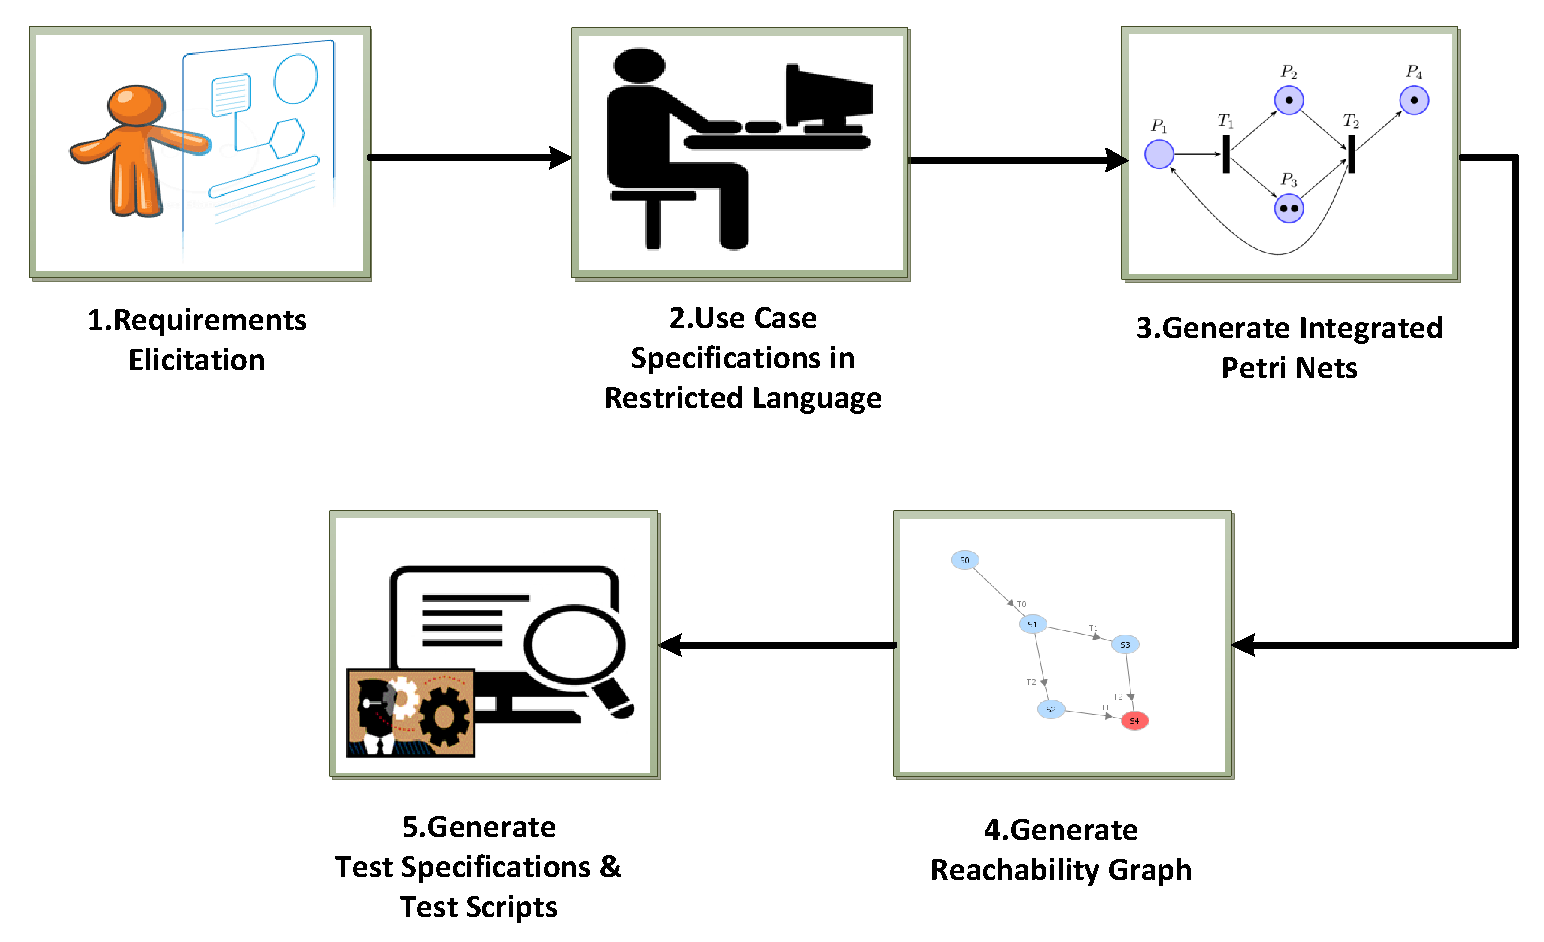
\includegraphics[width=0.9\textwidth]{content/images/Chapter1/proposed_solution.pdf}}
\caption{An overview of the proposed solution}
\label{fig:proposed_solution}
\end{figure}
\section{Thesis Management}
A project plan was created in order to guarantee an organized approach to this thesis work. Various milestones were created to monitor the progress of the project with time.
\subsection{Project Plan}
A Waterfall model with overlapping phases was created for project planning. The Gantt chart in Figure \ref{fig:gc} shows the various phases and the time duration planned for each phase. 
The significant phases are enlisted below.
\begin{enumerate}
\item Literature Survey
\item Design and Development
\item Testing and further development
\item Documentation
\end{enumerate}
From the Gantt chart, it can be seen some phases are overlapped. For example, the overall design of the approach and tool selection for implementation can be made immediately once a feasible approach has been identified in the literature survey. The identification of a suitable system and the enumeration of requirements for basic functionalities of the proposed tool can be done in parallel to the above mentioned phase.
\begin{figure}[htb!]
\centering
\fbox{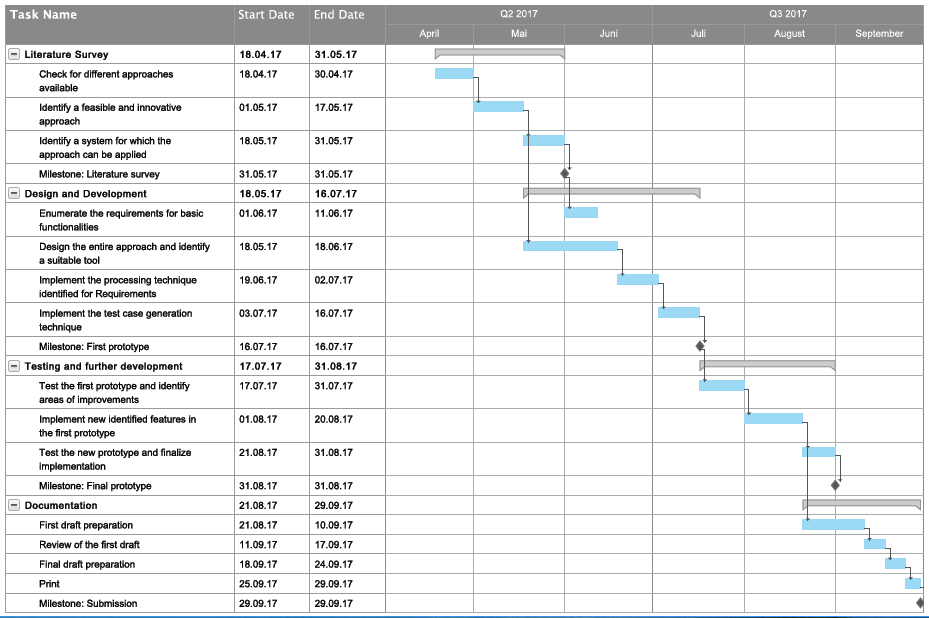
\includegraphics[scale = 0.69]{content/images/Chapter1/figure_2_ganntchart}}
\caption{Gannt Chart for the thesis work}
\label{fig:gc}
\end{figure}
\subsection{Literature Survey}
This thesis mainly revolves around the work done by Edgar et. al., 2015 \cite{sarmiento2015mapping}, Wang et. al., 2015 \cite{wang2015automatic} and Toa Yue et. al., 2015 \cite{yue2015rtcm}. The literature survey started with the books from the Library of University Stuttgart and moved towards online resources like the IEEE Xplore catalog, the ACM digital library, the E-Books from various publishers like Springer, the search engines from Internet such as Google\footnote{https://www.google.de} and specific search engines for scientific journals like Google Scholar\footnote{https://scholar.google.de}. Apart from the scientific journals and publications, numerous other resources had been used from the internet regarding the availability of different tools, their user manuals and their documentation.
\subsection{Thesis Structure}
The thesis has been organized as the following chapters.
\paragraph{Chapter 1} This chapter gives a short introduction to the thesis work, the motivation behind the thesis and a rough idea of the proposed solution.
\paragraph{Chapter 2} This chapter gives a short introduction to the different methodologies and terminologies that will be used throughout the rest of the thesis.
\paragraph{Chapter 3} This chapter provides an overview of related research work in the domain of automatic test case generation and it also gives a basic introduction to the technologies used in the implementation stage of the thesis.
\paragraph{Chapter 4} This chapter provides a detailed account of the proposed approach and the various methodologies used for test script generation.
\paragraph{Chapter 5} This chapter gives a deeper insight into the design of the tool and the implementation of the different methodologies introduced the previous chapter.
\paragraph{Chapter 6} This chapter illustrates the evaluation of the proposed tool and its comparison with other similar approaches.
\paragraph{Chapter 7} This chapter provides a short overview of the thesis and details the different limitations and contributions of the current work.
% !TeX spellcheck = de_DE
\chapter{Background}\label{background} 
This chapter gives a short introduction to topics regarding Agile processes and their definitions, Model Driven Architecture, Unified Modeling Language and Petri Nets. Basic knowledge in these topics helps us to appreciate the various design and implementation decisions taken in Chapter \ref{relatedwork} and \ref{proposedsolution}. This chapter also acts a guide to understand the various terminologies used throughout this work.

\section{Evolution of Agile Software Development}
Agile Software Development was introduced in the year 2001 by Agile Alliance to keep up with growing demands of the software industry. Traditional software development methods like Waterfall model couldn’t deliver the expected results on circumstances of frequent requirement changes and increased software complexity. The main reason that can be attributed to the failure of traditional development methods is the single flow of sequential development phases without any iterative phases.

For example, in Waterfall Model, the business analyst along with the client creates a set of requirements and a model of the final product. A requirement specification document is created which acts as the base document for the next development phases like Analysis, Design, Development and Testing of the product. The client is never involved during the development process and would view the product only after the final testing is completed. If the requirements of the client were not captured correctly or if the client has a changed requirement, then the entire development process has to be repeated. This kind of rework increases the cost, time and resources needed for the project and subsequently leads to its failure. (\cite{versionone}, \cite{getzephyr})

Agile Software Development, on the other hand, is built on the foundation of iterative approaches, in which product development happens incrementally and stakeholder participates in the entire \gls{sdlc} from the conception to the delivery of the product. One such methodology is \textit{Sprint} in which a larger functionality is broken into smaller pieces called \textit{User Stories} which can be delivered in a time span of just two weeks. This approach has several advantages such as the time consuming documentation is replaced with face to face communication with the stakeholders reducing the misinterpretation and hence a providing better understanding of stakeholder requirements.

Agile also provides separate methodologies for testing which makes testing easier with a quick feedback from stakeholders. A user story is marked complete if it passes all the acceptance tests. They are then evaluated whether to retain them for regression testing. A difference in interpretation of the requirement can be found out immediately with feedback and only a small rework will be needed in case of a difference. Test team members create the test plan, write test specifications and test cases and manage the testing activities within a sprint. The testing activities can be classified as follows.

\subsection{Requirements-Based Testing}
In this testing methodology, the objective is to verify whether the deliverables’ design and code meets the application’s requirements. Hence the test cases, conditions and data are generally derived from the requirements specification document. The testing can be done to verify either the functional attributes or the non-functional attributes like performance, reliability or usability. \cite{tahat2001requirement}

\subsection{Model-Based Testing}
This methodology involves the generation of test cases from models describing the system requirements and behavior. Even though this methodology requires the building of models up-front in the development cycle, it has several advantages like finding inconsistencies in the requirements itself and detection of discrepancies even before the code is generated. \cite{dias2007survey}

\subsection{Code-Based Testing}
In this methodology, test cases are used to evaluate the code to verify whether different test paths of the system are covered. The benefits of this methodology are that the parts of the software not tested in other techniques are covered. \cite{prasanna2005survey}

The main objective of this thesis is to simplify the existing test management process. As bulk of the effort is spent on elicitation and generation of test cases, this thesis aims to simplify the task of test case generation by using an automated tool. Most of the existing approaches for automated generation of test cases can be put under the above three categories. This thesis tries to automate test case generation for the first category which is Requirements-Based Testing.


\section{Model Driven Software Engineering}
An important paradigm shift happened in the field of software development after the introduction of \gls{mda} by \gls{omg}.   The underlying idea of \gls{mda} is to make use of models, a key tool in engineering, for software development. In general, models can be defined as abstraction of the system and its environment. An advantage with models is that it can be used to provide different levels of abstraction, with each level highlighting specific aspects or features of the system. Hence a model is essentially a representation of the necessary characteristics of the underlying system, leaving out the rest and thus contains less complexity. Less complexity of the models provides an easy way of system behavior prediction, examination of specific properties and unambiguous communication among software developers.

One of the motivations for \gls{mda} approach is that the developed software will be deployed to one or more platforms. The volatility of the platforms is higher than the higher-level models of the system and the objective of \gls{mda} is to create models that are increasingly independent of the target platform. In \gls{mda}, \glspl{pim} are initially designed in a platform independent language (e.g. \gls{uml}), which are then translated into \glspl{psm} by mapping them to some implementation language (e.g. C++, Java) as illustrated in Figure \ref{fig:Overview_MDA}.

\begin{figure}[htb!]
\centering
\fbox{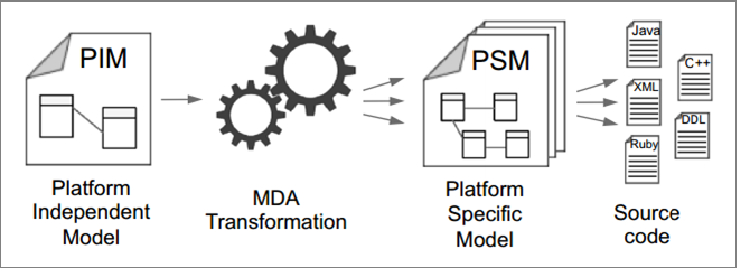
\includegraphics[width=0.8\textwidth]{content/images/Chapter2/Overview_MDA.pdf}}
\caption{Overview of transformations in MDA \cite{cerny2015separation}}
\label{fig:Overview_MDA}
\end{figure}

A number of \gls{omg} standards such as The \gls{uml}, \gls{xmi}, \gls{cwm}, \gls{mof} form the core of \gls{mda} concepts. Among these standards, \gls{uml} is used to define the \gls{pim} models which will be discussed in detail in the Section \ref{secuml} whereas the other standards are not in the scope of this thesis.

The term \gls{mdsd} or \gls{mdd} describes the family of engineering approaches that use models and their transformations for creating software products. \gls{mdsd} takes advantage of the \gls{mda} facilities, as a result of which the code can either be automatically or semi-automatically generated from models that are described in standard specification languages. The main priority of \gls{mdsd} is to enable the validation of software by the end users and customer stakeholders as early as possible in \gls{sdlc}.



\section{Unified Modeling Language} \label{secuml}
\gls{uml} is a standard from \gls{omg} and is a de-facto industry standard for modeling business applications in \gls{mdsd} \cite{cerny2015separation}. \gls{uml} models help to understand the requirements of the system graphically. They also provide aides to design the system, its components and to model the relationship existing between them right from early stages of software development. \gls{uml} also helps the developers and end users to maintain consistency in their interpretation of the design specification. \gls{uml}’s rapid gain in popularity in object oriented software development has attracted a great deal of research on \gls{uml} in software testing. (\cite{nebut2003requirements},\cite{badri2003use},\cite{nebut2003requirements})

\gls{uml} can be classified broadly into two categories namely structural and behavioral models. The structural diagrams represent the static structure of the system and the relationship between them. The different structural diagrams represent different abstraction and implementation levels. On the other hand, behavioral diagrams represent the dynamic behavior of the objects in the system i.e. the changes that happen in the system over time. Some of the important \gls{uml} diagrams which are used in upcoming sections are elaborated below.

Class Diagram is one example of structural diagrams that acts as a blueprint of the system or subsystem under development. It is extensively used to model the objects that make up the system, the relationship between them, their description and the functions they provide. Class Diagrams usage is across different levels in the development cycle. In analysis stage, it is used to understand the requirements of the problem domain whereas, in the implementation stage, it can be used to create actual software classes. An example of Class Diagram is shown in Figure \ref{fig:umldiagrams_subfigA}.

Activity Diagram is one example of behavioral diagrams which illustrates the sequence of actions in a process. Activity Diagrams usage across different levels in the development cycle are illustrated below. In requirements stage, it can be used to model the flow of events that the use cases describe and in design and implementation stage, it can be used to define the behavior of operations. An example of Activity Diagram is shown in Figure \ref{fig:umldiagrams_subfigB}.

\begin{figure}[htb!]
  \centering
    \subfloat[A UML Class Diagram]{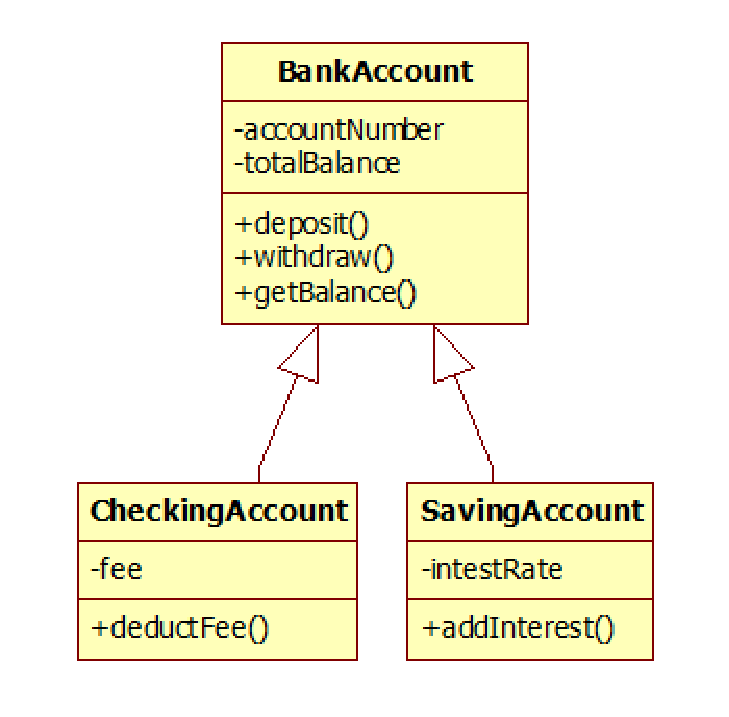
\includegraphics[width=0.45\textwidth,frame]{content/images/Chapter2/ClassDiagram.pdf} \label{fig:umldiagrams_subfigA}}
   \subfloat[A UML Activity Diagram]{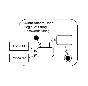
\includegraphics[width=0.45\textwidth,frame]{content/images/Chapter2/ActivityDiagram.pdf} \label{fig:umldiagrams_subfigB}}
	\caption{Examples of UML diagrams.}
\label{fig:umldiagrams}
\end{figure}

\section{Petri Net}
Petri Net is a graphical and mathematical modeling tool with well defined semantics suitable for formal analysis. The concept of Petri Net was first introduced by Carl Adam Petri in the year 1961, after which it had grown tremendously to support different domains like workflow management, manufacturing, real time systems, distributed systems, embedded systems, protocols and networks, performance evaluation and much more.
 
In the domain of computer science engineering, Petri nets are mainly used in information processing systems that can be categorized as parallel, concurrent, distributed, asynchronous, non-deterministic and stochastic. Petri nets can be used as communication documents like flow charts, block diagrams and networks but can also simulate the dynamic and concurrent activities of the system with the concept of tokens. Also, it can model the mathematical representations of the systems using algebraic and state equations. 

\subsection{Basics of Petri Net}
There are different kinds of Petri Nets depending upon the amount of information that the nets can carry. One such example of low level Petri Net is the Place/Transition Net (PT-Net) which is used in this thesis.

A Petri Net is an example of directed, bipartite and weighted graph in between two nodes called places and transitions. Arcs run between places and transitions and each place can hold specific items called tokens. An example Petri Net is shown in Figure \ref{fig:petrinet_example} and the various elements are elaborated below.

\begin{figure}[htb!]
\centering
\fbox{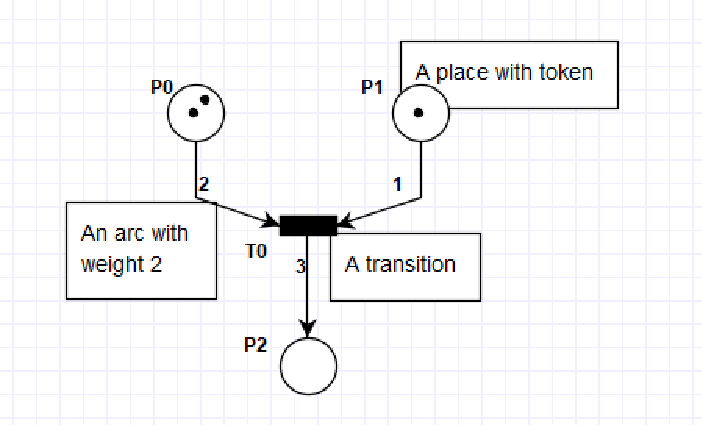
\includegraphics[width=0.6\textwidth]{content/images/Chapter2/Petrinetwithlabels.pdf}}
\caption{An example of Petri Net}
\label{fig:petrinet_example}
\end{figure}

\textbf{\textit{Places}} are the passive component of the net, and they represent the buffer, communication medium or in general a geographical location. The current state of the system is determined by the number of tokens present in a place and this state is represented by the term \textit{Marking} in Petri Nets.

\textbf{\textit{Transitions}} are the active components of the net, which represent the activities that change the state of the system. Transitions are fired only when certain preconditions are met and these conditions are represented in the net by means of tokens.

\textbf{\textit{Tokens}} are present inside the places and each token represents a condition to be fulfilled or a synchronization condition. In general, tokens represent a physical or information object.

\textbf{\textit{Arcs}} run only between places and transitions or vice versa. In the first case, these are called \textit{input arcs} whereas in the second case these are called \textit{output arcs}. Each arc is also associated with a specific weight that determines the number of tokens required for firing the particular transition.

\subsection{Formal Definition and Basic Terminology}
The terms defined in the above section can be formally defined as the following. The definitions are an excerpt from Calisaya et. al., 2015 \cite{calisaya2016analysis}.

\begin{definition}
\label{def:def1}
A \textbf{place-transition Petri Net} \cite{reisig2012petri}  is a five-tuple PN = (P, T, F, W, M$_{0}$) where P = $ \lbrace $p$_{1}$, p$_{2}$, ..., p$_{n} \rbrace $ is a finite set of places, T = $ \lbrace $t$_{1}$, t$_{2}$,..., t$_{n} \rbrace $ is a set of transitions, F   (P $\times$ T) $ \cup $ (T $\times$ P) is a set of arcs, W : F $ \subseteq $ $ \rightarrow$ $ \lbrace $1, 2,...$ \rbrace $ is a weight function, M$_{0}$ : P  $ \rightarrow\lbrace $0, 1, 2, ...$ \rbrace $ is the initial marking and P $ \cap $ T = $\emptyset $ and P $ \cup $ T 
$ \neq $ $ \emptyset $.
\end{definition}

\begin{definition}
\label{def:def2}
For a PN = (P, T, F, W, M$_{0}$), a \textbf{marking} is a function M: P $  \rightarrow$ $ \lbrace $0, 1, 2,...$ \rbrace $, where M (p) is the number of tokens in p. M$_{0}$ represents the initial marking of PN.
\end{definition}


\begin{definition}
\label{def:def3}
A \textbf{transition} t is enabled for firing at a marking M if M (p) $ \geq $ W (p, t) for any p $ \in $ p$ _{in} $ where p$ _{in} $ is the set of input places of t. On firing t, M is changed to M' such that $ \forall $p $ \in $ P: M' (p) = M (p) - W (p,t) + W (t,p). 
\end{definition}

\begin{definition}
\label{def:def4}
For a PN, a sequence of transitions $ \sigma $ = $ \langle $t$_{1}$, t$_{2}$, ..., t$_{n} \rangle $ is called a \textbf{firing sequence} if and only if M$_{0}$[t$_{1} \rangle $, [t$_{2} \rangle $,..., [t$_{n} \rangle $M$_{n}$. In notation, M$_{0}$ [PN, $ \sigma \rangle $M$_{n}$ or M$_{0}$ [$ \sigma \rangle $M$_{n}$.
\end{definition}

\begin{definition}
\label{def:def5}
For a PN = (P, T, F, W, M$_{0}$), a marking M is said to be \textbf{reachable} if and only if there exist a firing sequence $ \sigma $ such that M$_{0}$ [$ \sigma \rangle $M.
\end{definition}


\subsection{Analysis of Petri Nets}
One of the main features of Petri Net is the ability to perform analysis on model properties i.e. it can detect defects related to structural and dynamic properties \cite{murata1989petri}. A simple transversal of the flow relation between places and transitions can detect the structural properties whereas initial markings and final markings after transitions can detect the dynamic properties. As defined in \cite{reisig2012petri}, the defects due to dynamic properties of boundedness, liveliness, deadlock free and reachability can be detected using methods like simulation, reachability/coverability or invariant analysis.

 The transition behavior in a Petri Net is shown in Figure \ref{fig:petridiagrams}. Figure \ref{fig:petridiagrams} (a \& b) show Petri Nets with markings M0 and M1 respectively.  P0 and P1 are the places and T0 is the transition. The places contain tokens and arcs with arc weight of two and one respectively. This marking, which is the required precondition, enables the firing of the transition T0 and subsequently results in the marking as shown in Figure  \ref{fig:petrinet_subfigB}.  The final marking consists of place P2 with three tokens since the arc from T0 to P2 is of weight 3. 

\begin{figure}[htb!]
  \centering
    \subfloat[before transition]{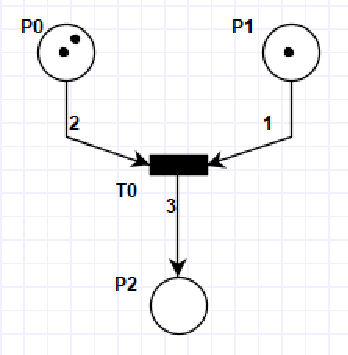
\includegraphics[width=0.4\textwidth,frame]{content/images/Chapter2/Petrineta.pdf} \label{fig:petrinet_subfigA}}
   \subfloat[after transition]{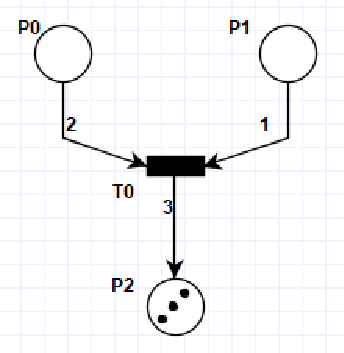
\includegraphics[width=0.4\textwidth,frame]{content/images/Chapter2/Petrinetb.pdf} \label{fig:petrinet_subfigB}}
	\caption{Concept of transitions in a Petri Net.}
\label{fig:petridiagrams}
\end{figure}



%\input{...weitere Kapitel...}
\input{content/kapitel2}
\input{content/zusammenfassung_und_ausblick}
%
%
%\renewcommand{\appendixtocname}{Anhang}
%\renewcommand{\appendixname}{Anhang}
%\renewcommand{\appendixpagename}{Anhang}
\appendix
\input{content/latex-tipps}

\clearpage

%\printindex

\printbibliography

\ifdeutsch
Alle URLs wurden zuletzt am 17.\,03.\,2008 geprüft.
\else
All links were last followed on September 20, 2017.
\fi

\pagestyle{empty}
\renewcommand*{\chapterpagestyle}{empty}
\Versicherung
\end{document}
